%! TEX root = diss.tex
\documentclass[../diss.tex]{subfiles}
\chapter{Implementation}

% NOTE: Multiprocessor => shared memory. Use term "parallel computer" instead

This chapter is empty, except for the inkscape figure shown in \autoref{fig:inkscape}.

\begin{figure}
\begin{center}
    % Note on inkscape figure: Use the \showthe\textwidth (and latexmk to see output
    %   and then create inkscape documents of that width when illustrating concepts!
    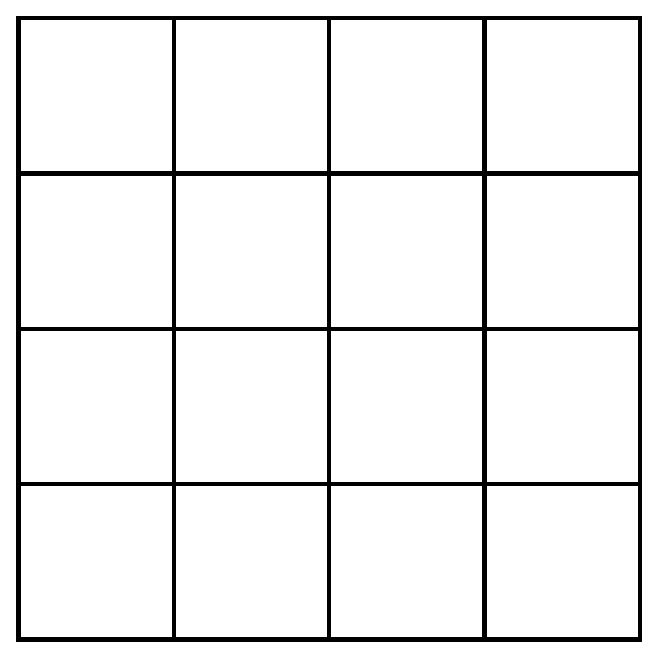
\includegraphics[scale=1]{figs/inkscape-example.eps}
\end{center}
\caption{An inkscape EPS diagram}
\label{fig:inkscape}
\end{figure}

% Introduction:
% * TODO: change fig 2.1 to have cloud of "graph data.csv" that interact with
%   "input graph"
% * Refer to figure 2.1, go into some more depth on interface to Parallel
%   system simulation:
%   * You create Worker implementation with access to ...., then pass
%     description to manager, specify number of workers, topology to use, num
%     computation phases, etc.
% * _Intrdc the different components, and then start going into detail in ind. subsecs_

% Some "practices used/software dev.? chapter":
% * Weekly meetings, log book, 

% Graph datasets:
% * California road networks:
%   * freely-available, consisten format, real-life road network
% * Random graphs:
%   * To satisyf req. of different n
%   * Erdos-Renyi graph, but modified to be fully-connected, trick to get same properties
%     with formula for creating $p$
%   *  python library used
% * Graph reader
%   * adjacency matrix and also neighbourhood list for Dijkstra's algorithm
% Graph datasets {{{
\section{Graph datasets}%
\label{sec:Graph datasets}

% }}}

% Simulation of a distributed memory multiprocessor:
% * Introduction:
% *   Overview of the components in bigger UML diagram, and comments on their interaction
% * TODO: create the above diagram first, and then realise what **more than below**
%         aspects to explain...
% * Memory model (?)
%   * explain design decision behind Map : (label : String) -> (value : Number)
%   * ...
% * Work management
%   * _By now, reader should know communication manager modifies memory when flush_
%   * Diagram of how work is simulated in parallel fashion, 8 blocks at a time
%   * Use Java's executor service to avoid thread management overhead
% * Worker factory
%   * Use of reflection, so can allow arbitrary description to be passed and can still
%     crete the new worker objects that can be managed
% * Timing analysis
%   * implemented as decorators for the system simulation
%   * Explain equations for how MIMD simulated (stalling bc. wait, latency+bandwidth etc.
%   * Repating computation measures, cache misses effect, possible bc.
%     seperation, mask read writes to ensure same computation done,
%     goal is more accurate eval
% Simulation of a distributed memory multiprocessor {{{
\section{Simulation of a distributed memory multiprocessor}%
\label{sec:Simulation of a distributed memory multiprocessor}

% }}}

% APSP via repeated matrix-squaring
% * Can abbriviate as MatSquare or something
% * Explain FoxOtto (explain predecessor functionality and edge-case,
%   generalized version, pseudo-code, diagram of memory movement can go in preparation)
% * Explain driver code, and its complexity?
% APSP via repeated matrix-squaring {{{
\section{APSP via repeated matrix-squaring}%
\label{sec:APSP via repeated matrix-squaring}

The \emph{\acl{MatSquare}} algorithm, which I will abbreviate as \emph{\acs{MatSquare}},
is an algorithm. \acused{MatSquare}
By using \ac{MatSquare}, we can ...
% }}}

% Graph compression:
% * The algorithm for this, and explain all the edge cases.
% * Also a section for the expected asymptotic speed-up referencing random graph generation
% Graph compression {{{
\section{Graph compression}%
\label{sec:Graph compression}

% }}}

% vim: foldmethod=marker
